\documentclass[UTF8]{ctexart}
\CTEXsetup[format={\Large\bfseries}]{section}
\usepackage{listings}
\usepackage{fontspec}
\usepackage{graphicx}
\usepackage{geometry}
\usepackage{amsmath}
\usepackage{palatino}
\usepackage{tikz}
\usepackage{xcolor}
\usepackage{listings}
\usepackage{xcolor}
\usepackage{algorithm}
\usepackage{algorithmicx}
\usepackage{algpseudocode}  
\usepackage{amsmath}
\usepackage{amsfonts}
\usepackage[justification=centering]{caption}
\usepackage{subfigure}
\usepackage{float}
\usepackage[super,square]{natbib}
\pagestyle{plain} %设置页眉页脚
\setmonofont{Consolas}
\lstset{
	language = python, numbers=left, 
	numberstyle=\tiny,keywordstyle=\color{blue!70},
	commentstyle=\color{red!50!green!50!blue!50},frame=shadowbox,
	rulesepcolor=\color{red!20!green!20!blue!20},basicstyle=\ttfamily
}

\usetikzlibrary{shapes.geometric, arrows}
\geometry{left=2.5cm, right=2.5cm, top=2.5cm, bottom=2.5cm}
\numberwithin{equation}{section}
\floatname{algorithm}{算法}
\renewcommand{\algorithmicrequire}{\textbf{输入:}}
\renewcommand{\algorithmicensure}{\textbf{输出:}}
\begin{document}
	\begin{center}  % 居中
		~\\:
		~\\:
		\huge
		哈尔滨工业大学计算机科学与技术学院 \\
		\Huge 
		实验报告 \\[5cm]
		\LARGE
		课程名称:机器学习 \\
		实验题目:PCA \\
		学号: \\
		姓名: \\
		\thispagestyle{empty}
		\clearpage  % 清除当页页码
	\end{center}
	
	\section{实验目的}
	实现一个$PCA$模型,能够对给定数据进行降维(即找到其中的主成分)
	\section{实验要求及实验环境}
	
	\subsection{实验要求}
	
	1. 首先人工生成一些数据(如三维数据),让它们主要分布在低维空间中,如首先让某个维度的方差远小于其它唯独,然后对这些数据旋转。生成这些数据后,用你的$PCA$方法进行主成分提取。
	
	2.找一个人脸数据(小点样本量),用你实现$PCA$方法对该数据降维,找出一些主成分,然后用这些主成分对每一副人脸图像进行重建,比较一些它们与原图像有多大差别(用信噪比衡量)。
	
	\subsection{实验环境}
	
	Python 3.7.4
	
	Pycharm
	
	\section{设计思想}
	
	\subsection{算法原理}
	主成分分析$(PCA)$经常用于数据降维,把数据投影到方差大的方向上,保留低阶主成分忽略高阶主成分,认为当数据方差大时,噪声的方差小,此时降维后的数据的信噪比较大。
	\subsubsection{基本思想}
	
	\begin{itemize}
		\item 将坐标轴中心移到数据的中心,然后旋转坐标轴,使得数据在$C1$轴上的方差最大,即全部$n$个数据个体在该方向上的投影最为分散。意味着更多的信息被保留下来。$C1$称为\textbf{第一主成分}
		\item $C2$\textbf{第二主成分}:找一个$C2$,使得$C2$与$C1$的协方差(相关系数)为$0$(协方差的特征向量,矩阵正交,两两垂直),以免与$C1$信息重叠,并且使数据在该方向的方差尽量最大。
		\item 以此类推,找到第三主成分,第四主成分。。。。第$p$个主成分。$p$个随机变量可以有$p$个主成分。
	\end{itemize}

	\subsubsection{证明}
	
	该证明参考《》机器学习(周志华著),给出两种等价的证明方法,最近重构性和最大可分性,此处给出最大可分性的证明。
	
	从最大可分性出发,得到出成分分析的解释。样本点$x_{i}$在新空间中超平面的投影是$\mathbf{W}^{T}x_{i}$,若所有样本点的投影能尽可能分开,则应该是投影后样本点的方差最大化。
	
	投影后样本点的协方差阵是$\sum_{i}\mathbf{W}^{T}x_{i}x_{i}^{T}\mathbf{W}$,于是优化目标可写为:

	\begin{equation}
	\begin{array}{cl}\max_{\mathbf{W}} & {\operatorname{tr}\left(\mathbf{W}^{\mathrm{T}} \mathbf{X} \mathbf{X}^{\mathrm{T}} \mathbf{W}\right)} \\
	{\text { s.t. }} & {\mathbf{W}^{\mathrm{T}} \mathbf{W}=\mathbf{I}}\end{array}\tag{1}
	\end{equation}
	
	该优化目标等价于
	
	\begin{equation}
	\begin{array}{cl}{\min _{\mathbf{W}}} & {-\operatorname{tr}\left(\mathbf{W}^{\mathrm{T}} \mathbf{X} \mathbf{X}^{\mathrm{T}} \mathbf{W}\right)} \\ {\text { s.t. }} & {\mathbf{W}^{\mathrm{T}} \mathbf{W}=\mathbf{I}}\end{array}\tag{2}
	\end{equation}
	
	对式$(2)$,其中,$\mathbf{X}=\left(\boldsymbol{x}_{1}, \boldsymbol{x}_{2}, \ldots, \boldsymbol{x}_{m}\right) \in \mathbb{R}^{d \times m}, \mathbf{W}=\left(\boldsymbol{w}_{1}, \boldsymbol{w}_{2}, \ldots, \boldsymbol{w}_{d^{\prime}}\right) \in \mathbb{R}^{d \times d^{\prime}}, \quad \mathbf{I} \in \mathbb{R}^{d^{\prime} \times d^{\prime}}$为单位矩阵。对于带矩阵约束的优化问题,可得到此优化目标的拉格朗日函数为:
	
	\begin{equation}
	\begin{aligned} L(\mathbf{W}, \Theta) &=-\operatorname{tr}\left(\mathbf{W}^{\mathrm{T}} \mathbf{X} \mathbf{X}^{\mathrm{T}} \mathbf{W}\right)+\left\langle\Theta, \mathbf{W}^{\mathrm{T}} \mathbf{W}-\mathbf{I}\right\rangle \\ &=-\operatorname{tr}\left(\mathbf{W}^{\mathrm{T}} \mathbf{X} \mathbf{X}^{\mathrm{T}} \mathbf{W}\right)+\operatorname{tr}\left(\Theta^{\mathrm{T}}\left(\mathbf{W}^{\mathrm{T}} \mathbf{W}-\mathbf{I}\right)\right) \end{aligned}\tag{3}
	\end{equation}
	
	其中,$\Theta \in \mathbb{R}^{d^{\prime} \times d^{d}}$为拉格朗日乘子矩阵,其维度恒等于约束条件的维度,且其中的每个元素均为未知的拉格朗日乘子,$\left\langle\Theta, \mathbf{W}^{\mathrm{T}} \mathbf{W}-\mathbf{I}\right\rangle=\operatorname{tr}\left(\Theta^{\mathrm{T}}\left(\mathbf{W}^{\mathrm{T}} \mathbf{W}-\mathbf{I}\right)\right)$为矩阵的内积,拉格朗日乘子矩阵$\Theta$为对角阵,令新的拉格朗日乘子矩阵为$\Lambda=\operatorname{diag}\left(\lambda_{1}, \lambda_{2}, \ldots, \lambda_{d^{\prime}}\right) \in \mathbb{R}^{d^{\prime} \times d^{\prime}}$,则新的拉格朗日函数为
	
	\begin{equation}
	L(\mathbf{W}, \Lambda)=-\operatorname{tr}\left(\mathbf{W}^{\mathrm{T}} \mathbf{X} \mathbf{X}^{\mathrm{T}} \mathbf{W}\right)+\operatorname{tr}\left(\Lambda^{\mathrm{T}}\left(\mathbf{W}^{\mathrm{T}} \mathbf{W}-\mathbf{I}\right)\right)\tag{4}
	\end{equation}
	
	对拉格朗日函数关于$\mathbf{W}$求导,令偏导等于$0$得:
	
	\begin{equation}
	\frac{\partial L(\mathbf{W}, \Lambda)}{\partial \mathbf{W}}=\frac{\partial}{\partial \mathbf{W}}\left[-\operatorname{tr}\left(\mathbf{W}^{\mathrm{T}} \mathbf{X} \mathbf{X}^{\mathrm{T}} \mathbf{W}\right)+\operatorname{tr}\left(\Lambda^{\mathrm{T}}\left(\mathbf{W}^{\mathrm{T}} \mathbf{W}-\mathbf{I}\right)\right)\right]=0\tag{5}
	\end{equation}
	
	得到
	
	\begin{equation}
		\mathbf{X X}^{\mathrm{T}} \mathbf{W}=\mathbf{W} \Lambda\tag{6}
	\end{equation}
	
	将$\mathbf{W}$和$\Lambda$展开可得:
	
	\begin{equation}
	\mathbf{X} \mathbf{X}^{\mathrm{T}} \boldsymbol{w}_{i}=\lambda_{i} \boldsymbol{w}_{i}, \quad i=1,2, \ldots, d^{\prime}\tag{7}
	\end{equation}
	
	于是,只需要对协方差矩阵$\mathbf{X} \mathbf{X}^{\mathrm{T}}$进行特征值分解,再将求得的特征值排序,取前$d'$大的特征值对应的特征向量构成$\mathbf{W}*$
	
	\subsubsection{高维数据的PCA}
	
	先考虑一维空间,假定一个单位向量$\boldsymbol{u}_{1}^{T} \boldsymbol{u}_{1}=1$。每个数据点$\boldsymbol{x}_{n}$被投影到一个标量值$u_{1}^{T} x_{n}$,则投影数据的方差为
	
	\begin{equation}
	\frac{1}{N} \sum_{n=1}^{N}\left\{\boldsymbol{u}_{1}^{T} \boldsymbol{x}_{n}-\boldsymbol{u}_{1}^{T} \overline{\boldsymbol{x}}\right\}^{2}=\boldsymbol{u}_{1}^{T} \boldsymbol{S} \boldsymbol{u}_{1}\tag{8}
	\end{equation}
	
	其中$\boldsymbol{x}$为样本均值,$S$为协方差矩阵
	
	\begin{equation}
	\begin{array}{c}{\overline{\boldsymbol{x}}=\frac{1}{N} \sum_{n=1}^{N} \boldsymbol{x}_{n}} \\ S=\frac{1}{N} \sum_{n=1}^{N}\left(\boldsymbol{x}_{n}-\overline{\boldsymbol{x}}\right)\left(\boldsymbol{x}_{n}-\overline{\boldsymbol{x}}\right)^{T}\end{array}\tag{9}
	\end{equation}
	
	现在最大化投影方差,引入拉格朗日系数来限制$\left\|u_{1}\right\| \rightarrow \infty$,记为
	
	\begin{equation}
	\boldsymbol{u}_{1}^{T} \boldsymbol{S u}_{1}+\lambda_{1}\left(1-\boldsymbol{u}_{1}^{T} \boldsymbol{u}_{1}\right)\tag{10}
	\end{equation}
	
	令关于$u_{1}$的导数等于$0$,我们看到方差为
	
	\begin{equation}
	\boldsymbol{u}_{1}^{T} \boldsymbol{S u}_{1}=\lambda_{1}\tag{11}
	\end{equation}
	
	推广到高维,此时协方差对应的特征向量方程为
	
	\begin{equation}
	\frac{1}{N} \boldsymbol{X}^{T} \boldsymbol{X} \boldsymbol{u}_{i}=\lambda_{i} \boldsymbol{u}_{i}\tag{12}
	\end{equation}
	
	进行变换得到
	
	\begin{equation}
	\left(\frac{1}{N} \boldsymbol{X}^{T} \boldsymbol{X}\right)\left(\boldsymbol{X}^{T} \boldsymbol{v}_{i}\right)=\lambda_{i}\left(\boldsymbol{X}^{T} \boldsymbol{v}_{i}\right)\tag{13}
	\end{equation}
	
	认为$v_{i}$的长度已经被归一化,为使$\left\|u_{i}\right\|=1$,有
	
	\begin{equation}
	u_{i}=\frac{1}{\left(N \lambda_{i}\right)^{\frac{1}{2}}} X^{T} v_{i}\tag{14}
	\end{equation}
	
	总结,为了应用$PCA$,首先计算$\boldsymbol{X} \boldsymbol{X}^{T}$,然后计算其特征值和特征向量,而后进行投影降维。
	
	\subsection{实现}
		\begin{algorithm}
			\caption{PCA}
			\begin{algorithmic}[1]
				\Require n维样本集$D=(x^{(1)}, x^{(2)}, \dotsc , x^{(n)})$
				\Ensure 降维后的数据集$D'$
				\Function {$PCA$}{$D$, $k$}
				\State 对所有样本去中心化
				\State 计算样本的协方差矩阵$XX^T$
				\State 对矩阵$XX^T$进行特征值分解
				\State 取出前$k$个最大的特征值对应的特征向量$(w_{1}, w_{2}, \dotsc , w_{k})$,将所有特征向量标准化后,组成特征向量矩阵$W$
				\State 对样本中的每一个样本$x_{(i)}$,转化为新的样本$z^{(i)} = W^{T}x^{(i)}$
				\State 得到输出样本$D'={z^{(1)}, z^{(2)}, \dotsc , z^{(k)}}$
				\EndFunction
			\end{algorithmic}
		\end{algorithm}
	
	\section{实验结果}
	
	\subsection{生成数据}
	
	\begin{figure}[htbp]
		\centering
		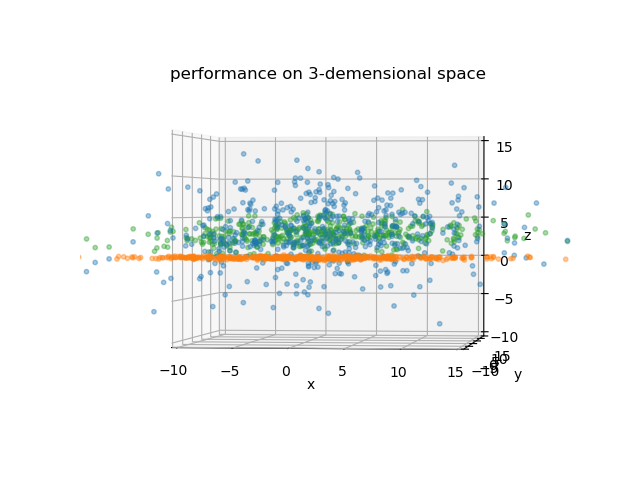
\includegraphics[scale=0.6]{Figure_1.png}
		\caption{生成数据降维示意图}
		\label{1}
	\end{figure}
	
	上图中蓝色为原始数据,橙色为降维后的数据,绿色为恢复数据,旋转可以看到数据都投影到了同一平面上,如下图所示。
	
	\begin{figure}[htbp]
		\centering
		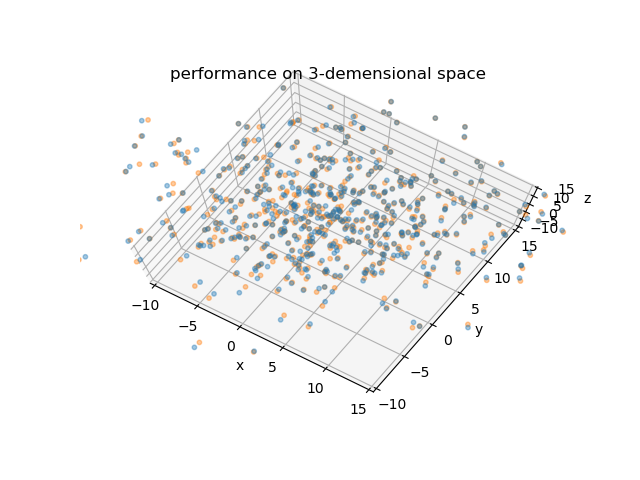
\includegraphics[scale=0.6]{Figure_2.png}
		\caption{投影到同一平面}
		\label{2}
	\end{figure}
	
	\subsection{人脸数据}
	
	使用的是$56*46$的人脸数据集,压缩图像与原图像对比如下图所示:
	
	\begin{figure}[htbp]
		\centering
		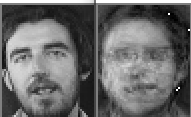
\includegraphics[scale=0.3]{1.png}
		\caption{人脸数据压缩对比(opencv)}
		\label{3}
	\end{figure}

	\begin{figure}[htbp]
		\centering
		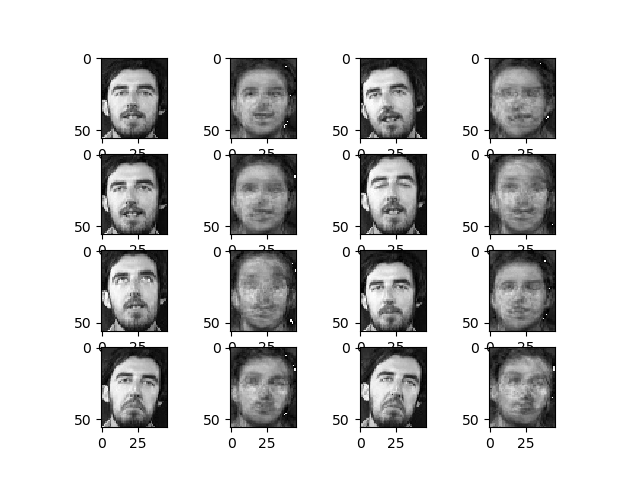
\includegraphics[scale=0.6]{Figure_6.png}
		\caption{人脸数据压缩对比(pyplot)}
		\label{3}
	\end{figure}
	
	将特征值打印出来可以发现,在第98个之特征值后特征值下降
	
	\begin{figure}[htbp]
		\begin{minipage}[t]{0.45\linewidth}
			\centering
			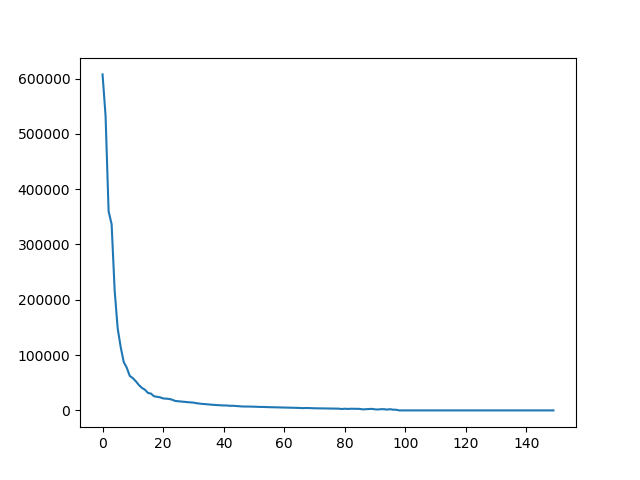
\includegraphics[height=4cm,width=6cm]{Figure_3.png}
			\caption{特征值曲线}
			\label{f1}
		\end{minipage}%
		\begin{minipage}[t]{0.45\linewidth}
			\centering
			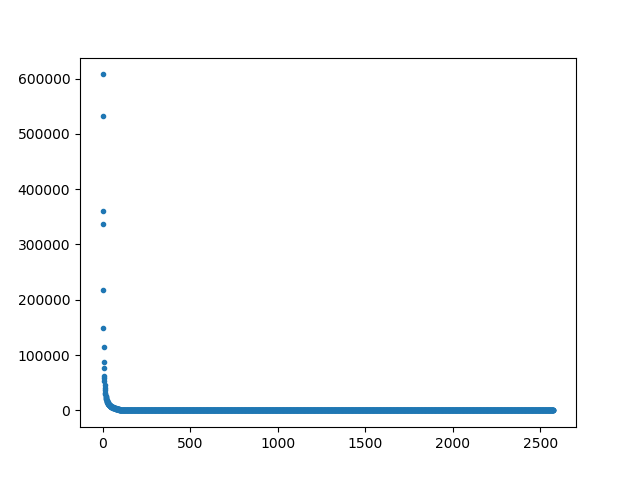
\includegraphics[height=4cm,width=6cm]{Figure_4.png}
			\caption{离散的特征值变化}
			\label{f2}
		\end{minipage}
	\end{figure}
	
	通过计算峰值信噪比$(PSNR)$,可以从数据层面看到压缩的质量,如下图所示:
	
	\begin{figure}[htbp]
		\centering
		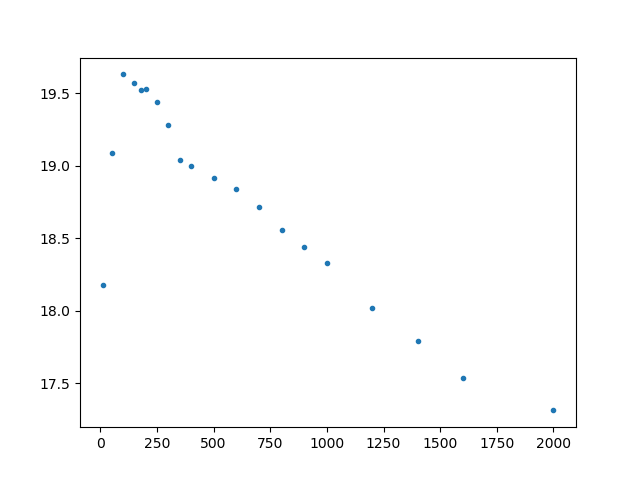
\includegraphics[scale=0.6]{Figure_5.png}
		\caption{PSNR}
		\label{3}
	\end{figure}
	
	\section{结论}
	
	\begin{itemize}
		\item $PCA$去掉的是方差较小的(不主要的信息),但不能保证去掉的是不重要的信息,因此$PCA$并不能解决过拟合现象,甚至可能加重了过拟合
		\item $ PCA $去除了噪声方差较大的数据,提高了信噪比,去除了冗余信息
	\end{itemize}
	
	\begin{thebibliography}{99}
		\bibitem{Tom} Tom M. Mitchell 《Machine Learning》
		\bibitem{Bishop} Christopher M.Bishop 《Pattern Recognition and Machine Learning》
	\end{thebibliography}
	\section{源代码}
	lab4.py
	\lstinputlisting {lab4.py}
	face.py
	\lstinputlisting {face.py}
\end{document}